\documentclass[12pt]{article}

\usepackage{fullpage}
\usepackage{multicol,multirow}
\usepackage{tabularx}
\usepackage{ulem}
\usepackage[utf8]{inputenc}
\usepackage[english, russian]{babel}
\usepackage{amsmath}
\usepackage{amssymb}
\usepackage{graphicx}

\usepackage{titlesec}

\titleformat{\section}
  {\normalfont\Large\bfseries}{\thesection.}{0.3em}{}

\titleformat{\subsection}
  {\normalfont\large\bfseries}{\thesubsection.}{0.3em}{}

\titlespacing{\section}{0pt}{*2}{*2}
\titlespacing{\subsection}{0pt}{*1}{*1}
\titlespacing{\subsubsection}{0pt}{*0}{*0}
\usepackage{listings}
\lstloadlanguages{Lisp}
\lstset{extendedchars=false,
	breaklines=true,
	breakatwhitespace=true,
	keepspaces = true,
	tabsize=2
}
\begin{document}


\section*{Отчет по лабораторной работе №\,3 
по курсу \\
\guillemotleft Функциональное программирование\guillemotright}
\begin{flushright}
Студент группы 8О-306 МАИ \textit{Наумов Дмитрий}, \textnumero 15 по списку \\
\makebox[7cm]{Контакты: {\tt dandachok@gmail.com} \hfill} \\
\makebox[7cm]{Работа выполнена: 27.04.2020 \hfill} \\
\ \\
Преподаватель: Иванов Дмитрий Анатольевич, доц. каф. 806 \\
\makebox[7cm]{Отчет сдан: \hfill} \\
\makebox[7cm]{Итоговая оценка: \hfill} \\
\makebox[7cm]{Подпись преподавателя: \hfill} \\

\end{flushright}

\section{Тема работы}
Последовательности, массивы и управляющие конструкции Коммон Лисп
\section{Цель работы}
Научиться создавать векторы и массивы для представления матриц, освоить общие функции работы с последовательностями, инструкции цикла и нелокального выхода.
\section{Задание (вариант №23)}
Запрограммировать на языке Коммон Лисп функцию, принимающую в качестве единственного аргумента двумерный массив, представляющий действительную матрицу A.

Функция должна возвращать новую матрицу B того же размера, каждый элемент которой bij равен сумме элементов матрицы A, расположенных в области, определяемой индексами i и j и заштрихованной на рисунке.

\begin{center}
    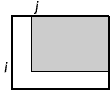
\includegraphics[scale=0.65]{arrays_matrix-ij-tr}
\end{center}

\section{Оборудование студента}
Процессор Intel Core i3-2100 4\,@\,2.2GHz, память: 8Gb, разрядность системы: 64.

\section{Программное обеспечение}
ОС Ubuntu 18.04.4 LTS, clisp 2.49.60

\pagebreak

\section{Идея, метод, алгоритм}
Алгоритм реализован в функции {\tt fun}.
Самая простая реализация - обычный перебор. Но лучше, для вычисления каждого элемента, использовать уже вычесленные, т.е. елемент $(i, j)$ результирующего массива будет равен сумме $(i - 1, j)$ и $(i, j - 1)$, при этом у нас дублируются элементы, которые лежат левее $j$-ого столбца и выше $i$-ой строки.
Поэтому надо вычесть $(i - 1, j - 1)$ элемент результирующего массива.

Так же есть вспомогательная функция {\tt copy-array}, котора создает копию массива.
\section{Распечатка программы и её результаты}
\subsection{Исходный код}
\begin{lstlisting} [language=lisp]
(defun copy-array (arr)
  (let* ((dimensions (array-dimensions arr)) (new-arr (make-array dimensions)))
    (dotimes (i (array-total-size arr))
      (setf (row-major-aref new-arr i)
            (row-major-aref arr i)))
    new-arr))

(defun fun (mat)
  (let ((size (array-dimensions mat)))
    (let ((lines (first size)) (columns (second size)) (ans (copy-array mat)))
      (do ((i 0 (+ i 1)))
        ((>= i lines) ans)
          (do ((j (- columns 1) (- j 1)))
            ((< j 0) 'done_str)
            (if (> i 0)
              (setf (aref ans i j) (+ (aref ans (- i 1) j)
                                    (aref ans i j))))
            (if (< j (- columns 1)) 
              (setf (aref ans i j) (+ (aref ans i (+ j 1))
                                   (aref ans i j))))
            (if (and (> i 0) (< j (- columns 1)))
              (setf (aref ans i j) (- (aref ans i j)
                                    (aref ans (- i 1) (+ j 1)))))
          )))))
\end{lstlisting}

\pagebreak

\subsection{Результаты работы}
\begin{lstlisting}
dandachok@dpc:~/Documents/Study/sem6/FP/lab3$ clisp
[3]> (load "solution.lisp")
;; Loading file solution.lisp ...
;; Loaded file solution.lisp
#P"/home/dandachok/Documents/Study/sem6/FP/lab3/solution.lisp"
[5]> (setq arr1 (make-array '(2 3) :initial-element 1))
#2A((1 1 1) (1 1 1))
[6]> (setq ans1 (fun arr1))
#2A((3 2 1) (6 4 2))
[7]> (setq arr1 (make-array '(3 4) :initial-element 2))
#2A((2 2 2 2) (2 2 2 2) (2 2 2 2))
[8]> (setq ans1 (fun arr1))
#2A((8 6 4 2) (16 12 8 4) (24 18 12 6))
\end{lstlisting}

\section{Дневник отладки}
\begin{tabular}{|c|c|c|c|}
\hline
Дата & Событие & Действие по исправлению & Примечание \\
\hline
\end{tabular}

\section{Замечания автора по существу работы}

\section{Выводы}
Алгоритм было просто придумать, благодаря дискретному анализу на 2-ом курсе, где мы проходили динамическое программирование.
Основные трудности возникли при реализации. Лисп менее удобен для изменения состояния переменных, чем другие языки программирования. Например, для изменения элемента массима требуется написать довольно длинную кострукцию.
\end{document}